\documentclass[11pt,a4paper]{article}
\usepackage[utf8]{inputenc}
\usepackage{amsmath}
\usepackage{amsfonts}
\usepackage{amssymb}
\usepackage{tikz}
\author{Mikkel Riber Bojsen - s093255}
\begin{document}
\section{$\mathcal{NP}$-completeness}

To prove $\mathcal{NP}$-completeness, we look at the problem \textsc{PartitionByPairs} (PBP). 

\subsection{Transformation}
Given an instance $X$ of PBP, we do the following transformation ($T(X)$). We calculate the value $B = \frac{\sum_{i=1}^{2n} s_i}{2}$. For each pair $(s_{2i-1}, s_{2i})$ in $S$,  where $i \in \lbrace 1,\dots, n \rbrace $, we construct a graph as show in Fig.~\ref{fig:transform1}, where the labels are the weights of the corresponding edge. 

\begin{figure}[!htb]
\centering
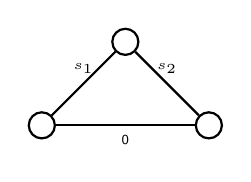
\begin{tikzpicture}[auto,node distance=1.5cm,
  thick,main node/.style={circle,draw,font=\sffamily\tiny\bfseries}]

  \node[main node] (1) {};
  \node[main node] (2) [above right of=1] {};
  \node[main node] (3) [below right of=2] {};
 % \node[main node] (4) [right of=3] {4};

  \path[every node/.style={font=\sffamily\tiny}]
    (1) edge node [above] {$s_1$} (2)
    	edge [right] node [below] {0} (3)
    (2) edge node [above] {$s_2$} (3);
    %	edge [bend left] node {0} (4)
   % (3) edge node {$s_2$} (4);

\end{tikzpicture}
\caption{Transformation of a single pair}
\label{fig:transform1}
\end{figure}

We order the set of edges, so the mirror of the edge with weight $s_{2i-1}$ is $s_{2i}$ and the mirror of an edge with weight 0 is an edge with weight 0 (if there is an odd number of pairs, the middle edge will be a zero that mirrors into itself). For multiple pairs, we chain multiple graphs together as shown in Fig.~\ref{fig:transform2}. 
\begin{figure}[htb]
\resizebox{\linewidth}{!}{
\centering
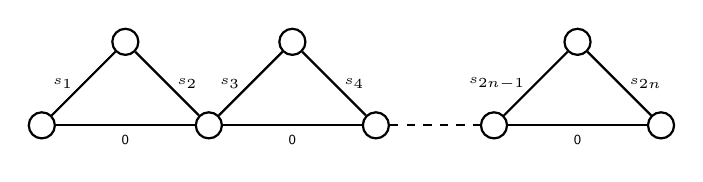
\begin{tikzpicture}[auto,node distance=1.5cm,
  thick,main node/.style={circle,draw,font=\sffamily\small\bfseries}]

  \node[main node] (1) {};
  \node[main node] (2) [above right of=1] {};
  \node[main node] (3) [below right of=2] {};
  \node[main node] (4) [above right of=3] {};
  \node[main node] (5) [below right of=4] {};
  \node[main node] (6) [right of=5] {};
  \node[main node] (7) [above right of=6] {};
  \node[main node] (8) [below right of=7] {};


  \path[every node/.style={font=\sffamily\tiny}]
    (1) edge node [left] {$s_1$} (2)
    	edge [right] node [below] {0} (3)
    (2) edge node [right] {$s_2$} (3)
    
     (3) edge node [left] {$s_3$} (4)
        	edge [right] node [below] {0} (5)
        (4) edge node [right] {$s_4$} (5)
    	
     (6) edge node [left] {$s_{2n-1}$} (7)
        	edge [right] node [below] {0} (8)
        (7) edge node [right] {$s_{2n}$} (8)
        
        ;
             
   \draw[style=dashed, ] (5) -- (6);
\end{tikzpicture}}
\caption{Transformation of several pairs}
\label{fig:transform2}
\end{figure}

For example, the set $S=\lbrace 1,2,3,4,5,6 \rbrace$ is transformed into a list of weights $W=[1,3,5,0,0,0,6,4,2]$, where the weight of edge $i$ is the $i$'th element in $W$.
\noindent
Using this graph and the calculated value $B$ we can query MFMST to answer PBP.

\subsection{Proof}

We do our transformation in polynomial time. The calculation of $B$ is done in $O(n)$. For each pair, we construct a constant number of nodes and edges, so the graph can be created in $O(n)$, this means our transformation can be done in $O(n)$.

If the answer to the original problem instance $X$ is YES, it means that a partition where we pick one from each pair equals $B$. It is possible to pick a spanning tree where we pick one from each pair as shown in Fig~\ref{fig:transform3}. As the answer to the original problem was YES, and we can pick a spanning tree that uses an edge from each pair, the answer must also be YES to $T(X)$.

\begin{figure}[htb]
\resizebox{\linewidth}{!}{
\centering
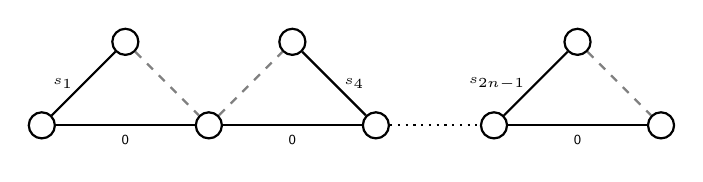
\begin{tikzpicture}[auto,node distance=1.5cm,
  thick,main node/.style={circle,draw,font=\sffamily\small\bfseries}]

  \node[main node] (1) {};
  \node[main node] (2) [above right of=1] {};
  \node[main node] (3) [below right of=2] {};
  \node[main node] (4) [above right of=3] {};
  \node[main node] (5) [below right of=4] {};
  \node[main node] (6) [right of=5] {};
  \node[main node] (7) [above right of=6] {};
  \node[main node] (8) [below right of=7] {};


  \path[every node/.style={font=\sffamily\tiny}]
    (1) edge node [left] {$s_1$} (2)
    	edge [right] node [below] {0} (3)
   % (2) edge node [right] {$s_2$} (3)
    
     (3) % edge node [left] {$s_3$} (4)
        	edge [right] node [below] {0} (5)
        (4) edge node [right] {$s_4$} (5)
    	
     (6) edge node [left] {$s_{2n-1}$} (7)
        	edge [right] node [below] {0} (8)
   %     (7) edge node [right] {$s_{2n}$} (8)
        
        ;
             
   \draw[style=dotted, ] (5) -- (6);
    \draw[color=gray, dashed] (2) -- (3);
        \draw[color=gray, dashed] (3) -- (4);
            \draw[color=gray, dashed] (7) -- (8);
\end{tikzpicture}}
\caption{A spanning tree}
\label{fig:transform3}
\end{figure}

We now assume the answer to the original problem is NO. In this case, we know that it is not possible to pick one edge from each pair in the transformation and get a value that is exactly $B$. 

Any spanning tree must pick at least one from each pair, but can pick two (ignoring the $0$-edge) and all edge weights are non-negative. 

If we pick more than one edge from a pair, we increase both the weight of the spanning tree and the mirror, as the two edges we pick are mirrors of each other, and therefore will be in both sums.

In summary, this means that if the original answer is NO, we cannot pick a spanning tree using one from each pair, where the maximum value of the tree and the mirror is exactly $B$. As we need to pick at least one from each pair to have a spanning tree, and picking more than one, always increases both values, we cannot get a spanning tree that will make MFMST answer NO.

As our transformation runs in polynomial time, the original problem is $\mathcal{NP}-complete$, our transformation preserves the original answer and MFMST is in $\mathcal{NP}$, we can conclude that MFMST is $\mathcal{NP}-complete$.

\end{document}